%!TEX root = ../main.tex

%fragment?
%students as our subjects

\section{Study setting}

Preprocessor-based SPLs may suffer modularity problems regardless of the VSoC support. When not using VSoC, we can see all feature code, being difficult to reason about the current task and focus on the target features. On the other hand, when using it, we hide feature code dependencies completely. In contrast, EIs do not hide everything. They abstract feature code details and, at the same time, provide information to support feature maintenance tasks.

To better understand the benefits and drawbacks of both approaches, we evaluate them by using controlled experiments. In particular, we investigate and compare maintenance effort when using VSoC and EIs and also count the number of errors that developers commit during maintenance tasks when using both approaches. So, we focus on \textbf{Effort} and \textbf{Errors} introduction.

\subsection{Goal, Questions, and Metrics}

To better structure our evaluation, we use the Goal, Questions, and Metrics (GQM)~\cite{basili-gqm-94} approach. Our evaluation aims to compare VSoC and EIs during maintenance tasks in preprocessor-based SPLs. We use VSoC because it provides benefits when compared to \texttt{\#ifdefs} purely~\cite{christian-second-chance-jot09}. The evaluation targets the developers point of view, involves undergraduate and MSc/PhD students with some professional experience, and observes effort and number of errors during maintenance tasks in preprocessor-based SPLs.

In particular, we investigate the following questions:

\begin{itemize}

	\item \textbf{Question 1:} \textit{Do Emergent Interfaces reduce effort during maintenance tasks involving feature code dependencies in preprocessor-based systems?}
	
	\item \textbf{Question 2:} \textit{Do Emergent Interfaces reduce the number of errors during maintenance tasks involving feature code dependencies in preprocessor-based systems?}

\end{itemize}

To answer \textbf{Question~1}, we use the following metric: \textit{Time} to complete a maintenance task. To better explain this metric, consider the \textbf{Scenario~1} presented in Figure~\ref{fig:arena-example}, where the developer should also take negative scores into account. \textit{Time} counts the amount of time needed to find feature dependencies (in our example, the use of \texttt{totalScore} in \textit{ARENA}) and to change the impacted features to accomplish the task. In our example, change means removing the ternary operator in the impacted feature (\textit{ARENA}) so that it accepts negative scores.

To answer \textbf{Question~2}, we use the following metric: Number of Errors (\textit{NE}) committed during a maintenance task. In this work, we consider \textit{error} as a human action that produces an incorrect result~\cite{ieee-se-glossary-90}. So, for each maintenance task, developers might commit errors. Still using \textbf{Scenario~1}, suppose that the developer did not remove the ternary operator. During our evaluation, if she submits she did accomplish this task, the \textit{NE} for this task is one. If she submits without removing the ternary operator again, \textit{NE} now is two for this task. In summary, \textit{NE} is the number of wrong submissions committed during a maintenance task. We also use the \textit{NE} metric to count wrong submissions for each task with respect to feature expressions. Using the \textbf{Scenario~2} as an example, suppose that the developer writes \texttt{\#ifdef (CHOWN)} to encompass \texttt{status}. Likewise, if she submits she did accomplish the task, the \textit{NE} for this task is one.

To investigate the research questions, we use $2$ preprocessor-based SPLs: a commercial one (\textit{Best Lap}) and an academic one (\textit{Mobile Media}).

\subsection{Hypotheses and Experiment Design}

In particular, we investigate the following hypotheses:

\begin{itemize}

	\item \textbf{H1:} When using VSoC and Emergent Interfaces, developers spend on average the same time to complete a maintenance task involving feature dependencies.

\begin{eqnarray}
\centering
\label{eq:h0}
H1_0 & : & \mu_{TimeVSoC} = \mu_{TimeEI} \\
\label{eq:h1}
H1_1 & : & \mu_{TimeVSoC} \neq \mu_{TimeEI}
\end{eqnarray}

	\item \textbf{H2:} When using VSoC and Emergent Interfaces, developers commit on average the same number of errors when performing a maintenance task involving feature dependencies.

\begin{eqnarray}
\centering
\label{eq:h0-errors}
H2_0 & : & \mu_{ErrorsVSoC} = \mu_{ErrorsEI} \\
\label{eq:h1-errors}
H2_1 & : & \mu_{ErrorsVSoC} \neq \mu_{ErrorsEI}
\end{eqnarray}

\end{itemize}

To evaluate these hypotheses, we need to define the experiment design. We opt for the Latin Square Design~\cite{box-statistics-for-experimenters}. To fit into this design, we select maintenance tasks based on two product lines (\textit{Best Lap} and \textit{Mobile Media}), since we have two treatments. In this design, we dispose subjects in rows and product lines in columns. The treatments come inside each cell in such a way that each treatment appears only once in every row and every column. Figure~\ref{fig:latin-squares} presents the layout of this design.

\begin{figure}[htp]
    \centering 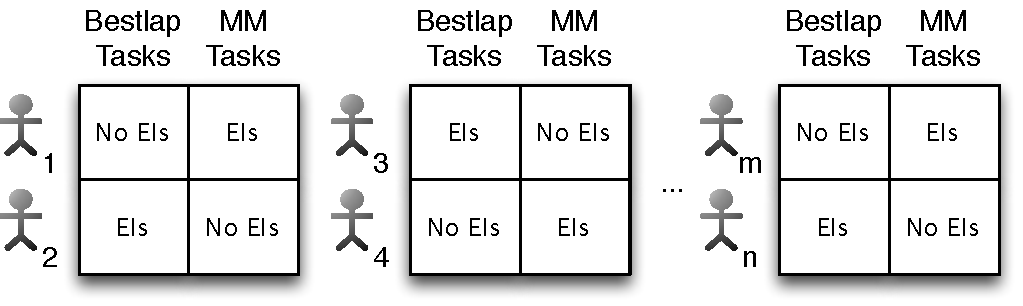
\includegraphics[width=0.4\textwidth]{images/Latin-squares.eps}
    \caption{Layout of our experiment design: latin squares.}
    \label{fig:latin-squares}
\end{figure}

As can be seen, each subject ($1, 2, ..., m, n$) performs maintenance tasks in each product line (\textit{Best Lap} and \textit{Mobile Media}) by using each technique (VSoC and Emergent Interfaces). This design is important to avoid undesirable effects such as learning. For example, if a developer uses both techniques in the same task, we would favor the second technique, since she already knows how to accomplish the task.

Therefore, the design we use blocks two factors: subject and maintenance tasks. This way, we do not favor any treatment.

\subsection{Experiment Instrumentation}

To carry on this design, we allocate each subject into one particular machine. To avoid the effect of software installed in different machines, we provide a virtual machine and install it in computers of similar hardware. In the virtual machine, we have $4$ Eclipses with the following configurations:

\begin{itemize}

	\item \textbf{Eclipse 1:} Emergo installed; \textit{Best Lap} imported;
	\item \textbf{Eclipse 2:} Emergo not installed; \textit{Best Lap} imported;
	\item \textbf{Eclipse 3:} Emergo installed; \textit{Mobile Media} imported;
	\item \textbf{Eclipse 4:} Emergo not installed; \textit{Mobile Media} imported.

\end{itemize}

Providing these $4$ Eclipses aims to reduce problems during the experiment execution. For example, if we provide only one Eclipse with everything, the subject might get confused and use the wrong technique in the wrong product line. Notice that each Eclipse represents one cell of our latin square design. We also have an additional Eclipse with Emergo installed and a toy product line imported (\textit{JCalc}, a simple calculator) for the experiment dry-run.

To collect the metrics automatically, we implemented an Eclipse plug-in. We install it in the four Eclipses, including the one we use for the dry-run. This plug-in consists of two buttons. The first one is a \textit{Play/Pause} button so that subjects can start/stop the time; and the second one is a \textit{Finish} button. So, before starting the maintenance task, the subject presses the \textit{Play} button. Then, the time is running. She can use this button to \textit{Pause} the time as well, which is important to ask questions during the experiment, for example.

Subjects press the \textit{Finish} button if they feel they accomplished the task. Our plug-in does not allow pressing this button when time is not running. When pressing it, we build the project and execute a test case. These steps take around $1$ second to execute in a contemporary laptop. We have one test case for each product line to verify if the subject accomplished a task correctly. If the test passes successfully, we stop the time and store this information in a file. Otherwise, the subject did not accomplish the task (the test has failed). This is therefore a wrong submission: the subject feels she accomplished the task, but actually she did not. So, the \textit{NE} for this task is one. In this case, if we consider that the \textit{Finish} button corresponds to a ``\textit{Submit to repository}" button in a real development environment, the subject would introduce a problem to the product line. Because we want to measure the time that subjects spend to accomplish exactly the same task, we do not stop the time in case the test does not pass. So, we ask the subject to continue the task until it passes.

Notice that we store the \textit{NE} metric result as well. We also use the Eclipse package explorer filters to hide the test cases. This is useful to forbid developers from seeing what is expected to accomplish the task. To implement VSoC, we use Eclipse projections, keeping the first line (the \texttt{\#ifdef} statement) to inform the subject that there is hidden code in such area.

To execute the experiment, we need to define the maintenance tasks. To better understand the effects of both techniques in different types of maintenance tasks, we consider the implementation of a \textbf{New requirement} and the fixing of \textbf{Unused variable} problems. They are different in the sense that the former takes \textit{interprocedural} feature dependencies into account. The latter, on the other hand, have only \textit{intraprocedural} dependencies: there is no dependency crossing the method boundaries when fixing an unused variable problem. We explain the \textbf{New requirement} tasks as follows.

For \textit{Best Lap}, the \textbf{New requirement} task is similar to the \textbf{Scenario 1} presented in Section~\ref{sec:incomplete}: let the game score be not only positive, but also negative. The variable that subjects should change is \texttt{score}. There is no \texttt{\#ifdef} statement encompassing it. We pass this variable as argument to two methods of the \texttt{NetworkFacade} class. These methods belong to the \textit{arena} feature and both contain a conditional statement forbidding negative scores by replacing them for zero. So, to accomplish the task, subjects should remove these conditional statements to allow negative scores.

For \textit{Mobile Media}, subjects should replace the actual web images server for another one that is able to provide more and different image formats. The variable they should change is \texttt{server}. Again, there is no \texttt{\#ifdef} statement encompassing it. We pass this variable to the \texttt{loadImage} method, which returns a random \texttt{image}. We then pass this variable to the \texttt{PhotoViewScreen} constructor, which uses the \texttt{image} in the \textit{zoom} feature. The zoom buttons are only available for vector formats. So, there is an \texttt{if} statement to verify the \texttt{image} format before adding the buttons into the screen. The new server returns a new vector format (\textit{PDF}). In this way, to accomplish the task, subjects should update the \texttt{if} statement to take this new vector format into consideration.

\subsection{Experiment Execution}

To make subjects aware of preprocessors, VSoC, feature dependencies, Emergent Interfaces, and Emergo, we provide training before running the experiment, which takes around $1$ hour. Our idea consists of providing a minimum knowledge so that all subjects can accomplish all tasks.

Regarding Emergo, we explain how to compute EIs and how to navigate throughout the code using it. Afterwards, we explain the buttons \textit{Play/Pause} and \textit{Finish}. We also discuss the target product lines (\textit{Best Lap} and \textit{Mobile Media}) but we do not present any code of these product lines. Finally, we inform them they sometimes use Emergo and sometimes they do not.

After training, we distribute \textbf{New requirement} and \textbf{Unused variable} maintenance tasks based on the \textit{JCalc} toy product line. We write them in the same way we present in Figure~\ref{fig:maintenance-tasks}. Then, we execute the dry-run simulating the experiment, so subjects use Emergo, projections that implement the VSoC idea, and the buttons exactly as if they are executing the experiment for real.

Then, we execute the experiment. In particular, in this work we consider three executions. All took around $2$ and half hours (training, dry-run, and execution). The \textbf{Pilot} had several problems, so we do not report its results. The subsequent executions---\textbf{Round~1} and \textbf{Round~2}---took place in two different universities. The first one considers MSc/PhD students whereas the second one considers undergraduate students. As mentioned, some of them have professional experience.